% Copyright � 2015 by James Dean Mathias
% All Rights Reserved

\chapter{Scalability - Fault-Tolerant}\label{chapter:ft}

Some systems require reliable computational results even when the computing environment itself is unreliable. For example, a company that deploys large data centers, comprised of hundreds or thousands of computers can reasonably expect one of these computers to fail on a daily, weekly, or monthly basis. It isn't reasonable for the data center to stop operation while the single faulty system is replaced. Furthermore, it isn't reasonable for whatever computation is currently taking place to have to be restarted because one of the computers failed during the execution. In order to overcome these failure scenarios, one or more strategies must be implemented that allow for graceful recovery. The general category of these strategies is known as \textit{Fault-Tolerance}.

Fault-tolerance is often, but not exclusively, discussed in terms of an unreliable computing environment, with the causes for that unreliability coming from any number of sources. For the work presented in this book I want to narrow, somewhat, the focus of the purpose for adding fault-tolerance to our system. The kind of computing environment I have in mind isn't necessarily unreliable, but rather dynamic in nature, growing and shrinking over time. For example, someone may desire to harness the computing power of systems when not in use during regular work hours, utilizing them in the evenings when no one is working. In order to do this, one needs to have the ability to dynamically add new systems as they become available later in the evening (this capability already demonstrated in Chapter \ref{chapter:dist}), but also gracefully (i.e. not lose work) handle systems that terminate unexpectedly when the regular daytime user logs on. While this is technically an unreliable network of computing resources, it is better thought of as a dynamic environment.

\section{Introduction}

What is fault-tolerance? The subject is broad, far too broad to reasonably cover comprehensively in this book. Instead this section offers a short introduction to the subject, enough to give a sense of the broader subject while focused enough to make sense out of the code presented as the primary part of this chapter.

A good definition of fault-tolerance is continued operation even when some part of the system fails, another is graceful degradation through redundancy. Generally speaking the intention with fault-tolerance is to acheive the following:

\begin{itemize}
	\item No single point of failure
	\item Fault isolation
	\item Fault containment
	\item Recovery
\end{itemize}

No single point of failure indicates that no individual system failure can bring the whole to a stop. Achieving no single point of failure is the most challenging part of a fault-tolerant system, the example provided in this chapter gets close, but doesn't fully meet this goal (a future book will present a system that fully acheives this goal). Fault isolation is the ability to isolate the system component responsible for the failure; this may come about through modular system design, failure detection mechanisms, or other means. Fault containment is the concept of not allowing the failure of one system component to propagate throughout the rest of the system. Recovery is the ability for a system to detect a failure has occured and continue correct operation in the face of that failure; this may mean rerouting requests originally sent to a failed component to another component that can complete the request.

How fault-tolerance is acheived comes through a variety of means. A short list of building blocks for fault-tolerance includes:

\begin{itemize}
 	\item Redundancy (space and time)
 	\item Atomic operations or transactions
 	\item Acceptance tests or voting
 	\item Data encoding
 	\item Algorithm diversity
 	\item Multiple correct results
 	\item Elections
\end{itemize}

Which of these building blocks are used depends upon the requirements of the fault-tolerant system. The most common building block, and the one used in this book, is redundancy. With respect to ease of system design, it is relatively easy to add multiple hard drives versus some other means to overcome the failure of a hard drive. This tends to hold true with other kinds of redundancy. It is fairly straightforward to duplicate resources, making it a popular choice. Other building blocks such as voting, elections, algorithm diversity, and multiple correct results require much more complexity to be added to the system, therefore they tend to be less frequently utilized.

As with everything else, fault-tolerance does not come for free, there are associated costs. The most obvious of these is money. Duplicated hardware costs money, as does duplicated effort to provide multiple implementations of the same algorithms to achieve algorithm diversity. While some things may only cost money (it might be possible to hire multiple engineers to develop multiple algorithms at the same time) it is usually the case that adding fault-tolerance also costs calendar time. A system that has a single algorithm for computing results is less complex than a system that uses multiple algorithms and compares those results before continuing. Not all parts of the more complex system can be implemented in parallel. It is simply going to take more time to develop the multiple algorithm system due to its greater complexity, resulting in a longer time to develop and deploy the system. Futhermore, adding fault-tolerance increases a system's complexity, making it more difficult to design, develop, and maintain.

A few examples of everyday system components that include fault-tolerance as part of their design include: TCP, error-correcting code memory (ECC memory), and RAID. TCP communication is designed with unreliable networks in mind, while providing a \textit{guarantee} of reliable communication. ECC memory is capable of detecting and correcting common kinds of data corruption. Some features of RAID provide for fault-tolerance through the use of redundancy and/or additional error detecting and correcting bits. These examples are not full systems in and of themselves, but represent real-world building blocks upon which a fault-tolerant system may be constructed. Looking back on the previous chapter's use of TCP for communication within the distributed system, we already see the use of fault-tolerance in the system without having to make any special effort.

It is important to note that fault-tolerance is just that and nothing more, it is not \textit{fault-proof}. A fault-tolerant system is designed to handle some classes or specific types of failure, but is not resistant to all failures. The degree to which a system is resiliant in the face of failures owes much to the resources (i.e. money and time) available to design and build aspects of fault-tolerance into the system.

\section{System Design}\label{chapter:ft:system-design}

The class of fault-tolerance added to the system for this chapter is that of tolerance to unexpected failures in the compute servers. When a compute server fails, for any reason, the whole system must gracefully handle the failure. Consider that a compute server may be in the middle of working on a task for the client when it fails. The system must recognize this failure and redirect that task to another compute server in order to ensure that all computations are completed. Furthermore, it is desired to contain this failure detection and task redirection logic to the core system components, making it as transparent to the application code as possible.

The fundamental system model does not change that much from the previous chapter, as shown in \FigureGeneral \ref{chapter:ft:model-figure}. The only new addition is that of an \textit{Assigned Work} set. Even though this is an apparently small change, its impact on the implementation is more than trivial, as will be seen in the remainder of this chapter.

\begin{figure}[H]
	\centering	
	\fbox
	{
		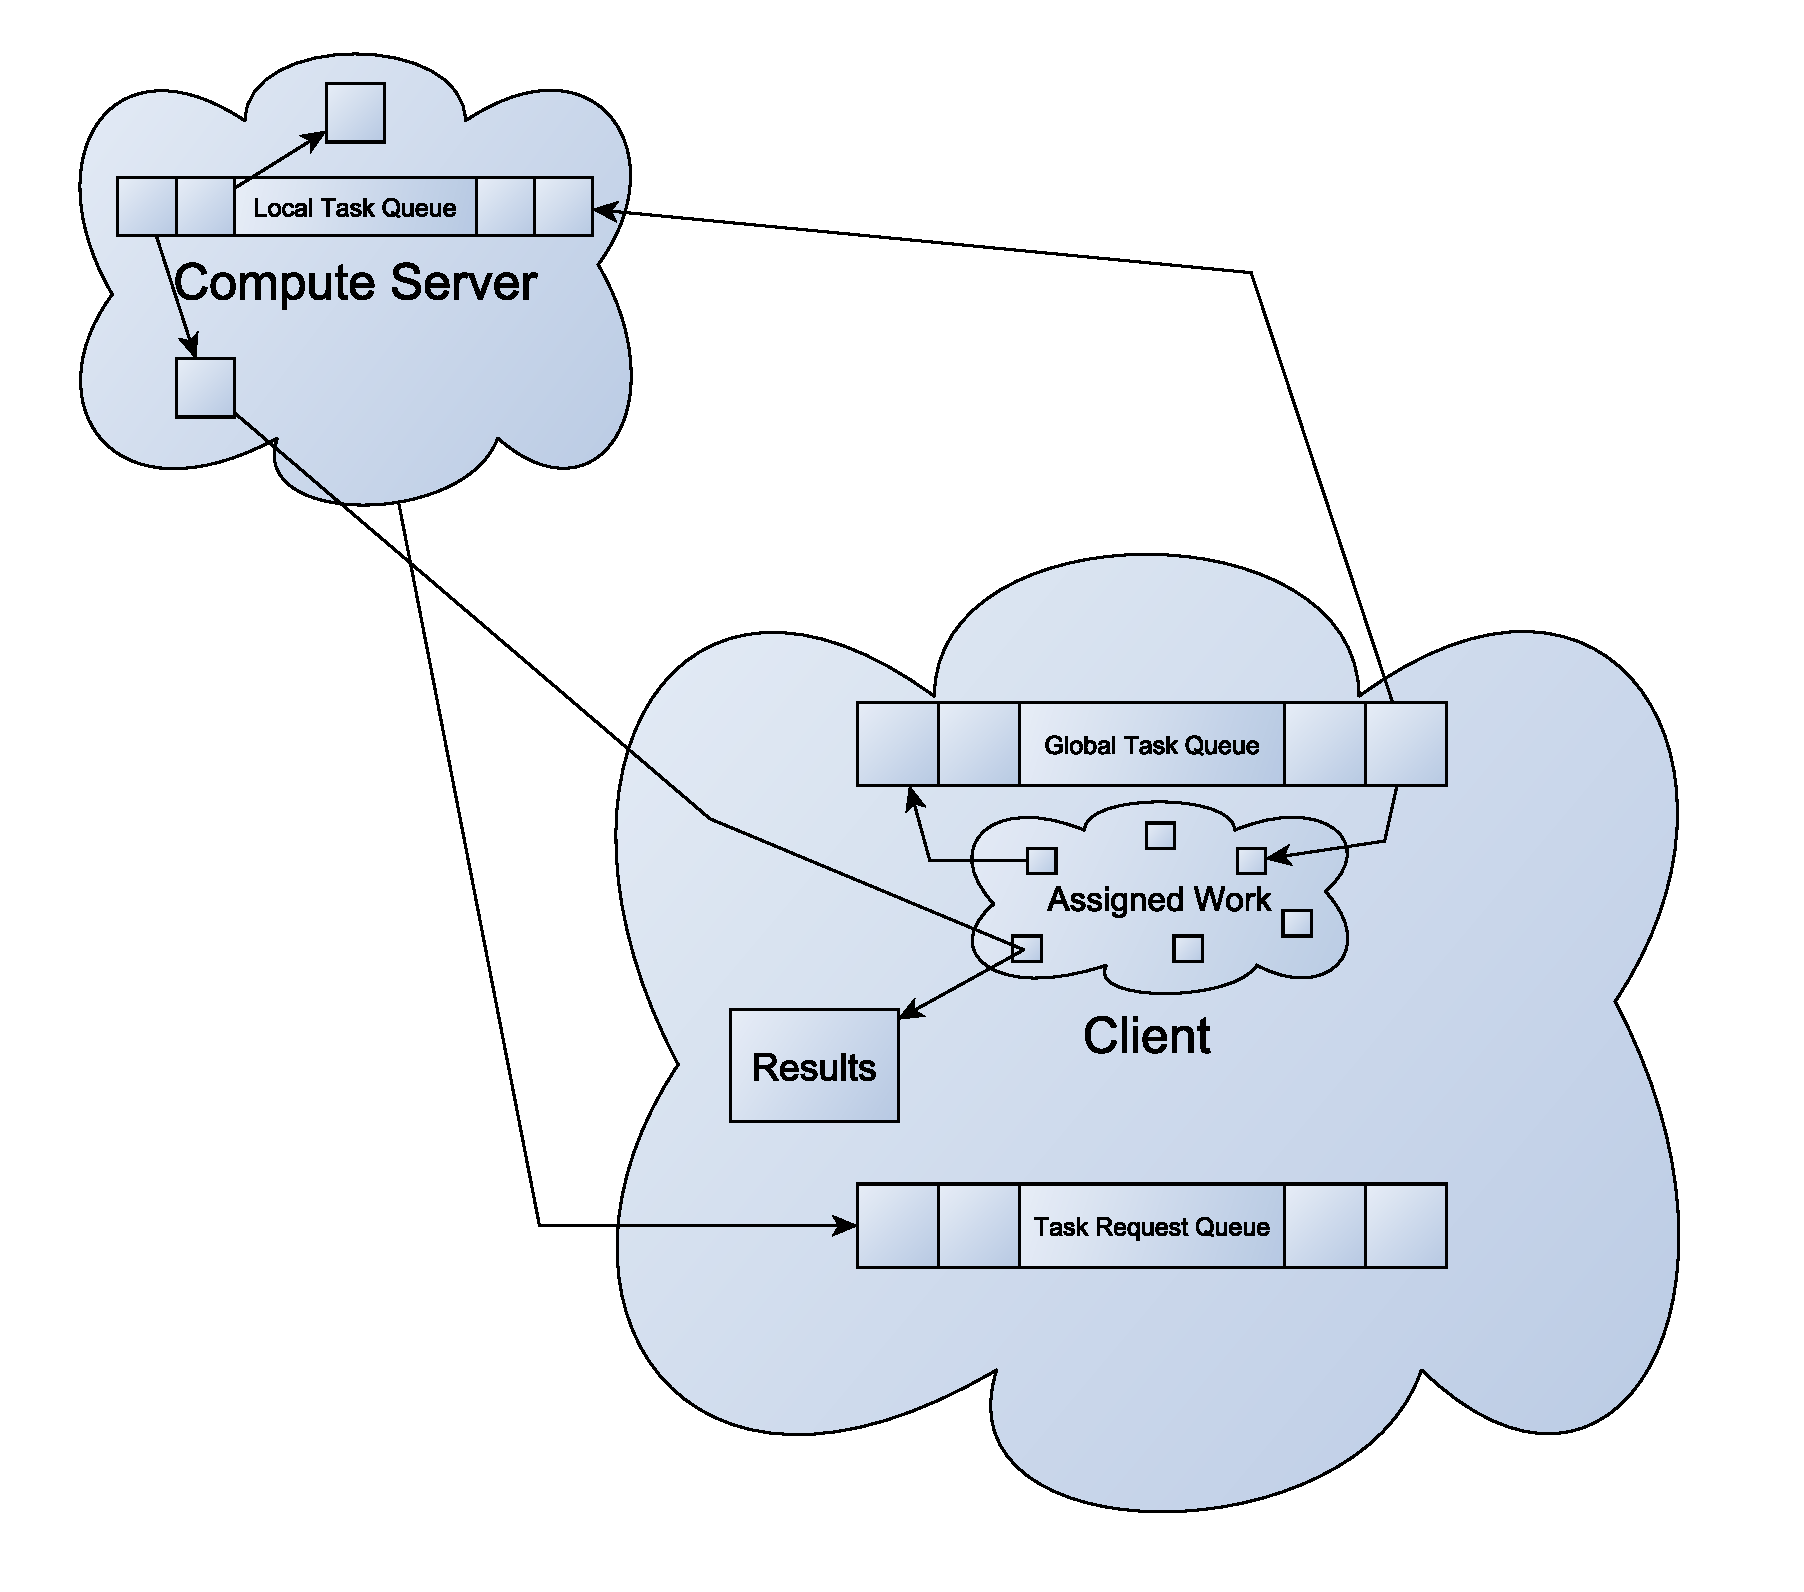
\includegraphics[width=4.5in, height=4.5in]{Images/FaultTolerant-Model.pdf}
	}
	\caption{Fault-Tolerant Model}
	\label{chapter:ft:model-figure}
\end{figure}

The purpose of the Assigned Work set is to have a way of identifying tasks that have been sent out for computation, but have not yet had their results returned. When a task is distributed to a compute server, that task is placed into the Assigned Work set, and given a maximum time in which a result is expected. In the normal case, when no failure has occurred, and when the task results are returned to the client, the task is removed from the Assigned Work set. In the failure case, the system periodically examines the Assigned Work set for any tasks that have not completed in their expected time and returns them to the Global Task Queue to match them with a new task request and sent back out for computation at a new compute server.

This change in the logic of the core client system to handle server failures, along with the existing ability to dynamically add new servers, is what allows the system to gracefully grow or shrink as computing resources come and go. With this model, we have now achieved the goal of a scalable, distributed, and fault-tolerant system. It is scalable in that it takes advantage of new computing resources, both CPU cores and distributed, is distributed, and can handle failures of connected servers.

I acknowledge the system has an important single point of failure at the client. If the client fails, the entire system fails. The solution to this is going to take a lot more work and is beyond the intended scope of this book. A future book is going to tackle this problem in a comprehensive manner.

\section{Framework Changes}\label{chapter:ft:section:framework-changes}

Based upon the new system model presented in Section \ref{chapter:ft:system-design}, various updates and additions to the core system framework have been implemented. In some places, such as the \texttt{Task} class, the changes are almost trivial, but in other places, such as the \texttt{TaskRequestQueue} the changes are more significant. Each of the core systems touched as part of adding fault-tolerance to the system is discussed in this section.

Before moving into the discussion of what is changed, it is useful to highlight the parts of the system that have seen no changes. Essentially everything about the server remains untouched. This includes the \texttt{ThreadPool}, the \texttt{TaskRequest}, and the \texttt{WorkerThread}. The entire networking infrastructure and message communication framework is untouched. The \texttt{Task} class is slightly modified, described in Section \ref{chapter:ft:section:task-update}, but not in a way that affects the server. Even though adding (server failure) fault-tolerance to the system is a big deal, the changes are actually localized to the client and do not impact the server.

\subsection{Updated \texttt{Task}}\label{chapter:ft:section:task-update}

\FigureGeneral \ref{chapter:ft:task-class} shows only the code associated with the updates to the \texttt{Task} class. A new \texttt{m\_duration} class member is added that represents the maximum amount of time it is expected for this task to be computed. The purpose of this duration is for failure detection. If the results for the task are not returned within this duration, a failure is detected and the task resubmitted to another server for computation. The constructor is updated to accept the duration parameter, with the expectation the derived classes set it to a value that is meaningful for the task. Finally, a new \texttt{getDuration} helper method is added to allow read-only access to the task duration.

\begin{code}[caption={Updated \texttt{Task} Class}, label=chapter:ft:task-class]
class Task
{
public:
  Task(std::chrono::milliseconds duration, Priority priority = Priority::One);

  std::chrono::milliseconds getDuration() const
  {
    return m_duration;
  }

private:
  std::chrono::milliseconds m_duration;
};
\end{code}

As a reminder, only the changed/added parts of the \texttt{Task} class are shown, all other parts of the class remain, but are not shown in the listing in order to help highlight the changes.

\subsection{New \texttt{AssignedTask}}\label{chapter:ft:section:assigned-task}

In order to identify which tasks have been distributed for computation, but have not yet returned a result, a new state (and container) is needed for tasks. The \texttt{AssignedTask} class is used as a wrapper around \texttt{Task} instances and held in a new container in the \texttt{TaskRequestQueue}. This wrapper contains a pointer to the original task, along with a deadline by which the result is expected before the task computation is considered to have failed. The declaration for the class is found in \FigureCode \ref{chapter:ft:assigned-task-class}.

\begin{code}[caption={\texttt{AssignedTask} Class}, label=chapter:ft:assigned-task-class]
class AssignedTask
{
public:
  explicit AssignedTask(std::shared_ptr<Tasks::Task> task);

  std::shared_ptr<Tasks::Task> getTask()
  {
    return m_task;
  }
  std::chrono::time_point<std::chrono::high_resolution_clock> 
    getDeadline() const 
    {
      return m_deadline;
    }

private:
  std::shared_ptr<Tasks::Task> m_task;
  std::chrono::time_point<std::chrono::high_resolution_clock> m_deadline;
};
\end{code}

When an instance of this class is created, the constructor, shown in \FigureCode \ref{chapter:ft:assigned-task-constructor}, takes the current time (\texttt{now}) and adds the task duration to it in order to come up with the deadline for when the task should have returned a result. This deadline is stored in the \texttt{m\_deadline} member of the class.

\begin{code}[caption={\texttt{AssignedTask} Constructor}, label=chapter:ft:assigned-task-constructor]
AssignedTask::AssignedTask(std::shared_ptr<Tasks::Task> task) :
  m_task(task)
{
  std::chrono::time_point<std::chrono::high_resolution_clock> now = 
    std::chrono::high_resolution_clock::now();
  m_deadline = now + task->getDuration();
}
\end{code}

When the \texttt{AssignedTask} instances are stored in a ordered container, a \texttt{std::priority\_queue} in our case, a means by which they can be sorted by their deadline is necessary. Therefore, the \texttt{AssignedTaskCompare} class shown in \FigureCode \ref{chapter:ft:assigned-task-compare} is necessary. This class overload the parenthesis \texttt{()} operator, taking two \texttt{AssignedTask} instances and returning a \texttt{true/false} depending upon which one is greater than the other. When the \texttt{std::priority\_queue} is declared in the \texttt{TaskRequestQueue}, this class is specified as the comparison functor. Using this scheme makes it possible to easily know which tasks have gone past their deadline; how this is done is discussed in futher detail in Section \ref{chapter:ft:section:task-request-queue}, which details the updated \texttt{TaskRequestQueue}.

\begin{code}[caption={\texttt{AssignedTaskCompare} Class}, label=chapter:ft:assigned-task-compare]
class AssignedTaskCompare : 
  public std::binary_function<
    std::shared_ptr<AssignedTask>,
    std::shared_ptr<AssignedTask>, bool>
{
public:
  bool operator()(
    const std::shared_ptr<AssignedTask> lhs, 
    const std::shared_ptr<AssignedTask> rhs) const
  {
    return (lhs->getDeadline() > rhs->getDeadline());
  }
};
\end{code}

\subsection{Updated \texttt{TaskRequestQueue}}\label{chapter:ft:section:task-request-queue}

The most significant changes to the code take place in the \texttt{TaskRequestQueue} class. \FigureCode \ref{chapter:ft:task-request-queue} shows the additions to the class; everything else presented in Chapter \ref{chapter:dist} remains part of the class, however with some of the method implementations changed. As noted before, the server code is essentially unchanged. It is the client code where the fault-tolerance logic was added, resulting in the large changes to the \texttt{TaskRequestQueue} class. Each of these additions, and changes to existing methods, is detailed next.

\begin{code}[caption={Updated \texttt{TaskRequestQueue}}, label=chapter:ft:task-request-queue]
class TaskRequestQueue
{
public:
  bool finalizeTask(uint32_t id, bool forceRemove);

private:
  std::priority_queue<
    std::shared_ptr<AssignedTask>,
    std::vector<std::shared_ptr<AssignedTask>>, 
    AssignedTaskCompare> m_queueAssigned;
  std::unordered_map<uint32_t, std::shared_ptr<AssignedTask>> m_mapAssigned;
  std::recursive_mutex m_mutexAssigned;

  void compactQueueAssigned();
  bool isQueueAssignedEmpty();
  void popQueueAssigned();
  bool mapAssignedContains(uint32_t id);
  boost::optional<std::shared_ptr<AssignedTask>> getQueueAssignedTop();
};
\end{code}

Let's start by looking at the updated \texttt{distribute} method in \FigureCode \ref{chapter:ft:distribute}. While looking at the revised \texttt{distribute} method, refer back to Chapter \ref{chapter:dist} and \FigureCode \ref{chapter:dist:trq:distribute} for the orginal implemention to get a better sense of the scope of the changed logic.

\begin{code}[caption={Updated \texttt{distribute} Method}, label=chapter:ft:distribute]
while (!m_distributerDone)
{
  Tasks::Task::Priority currentPriority = m_priority;
  bool donePriority = false;
  while (!m_distributerDone && !donePriority)
  {
    bool distributed = false;
    std::shared_ptr<Tasks::Task> task;

    compactQueueAssigned();

    if (!isQueueAssignedEmpty())
    {
      auto top = getQueueAssignedTop();
      if (top)
      {
        std::chrono::time_point<std::chrono::high_resolution_clock> now = 
          std::chrono::high_resolution_clock::now();
        if (top.get()->getDeadline() <= now)
        {
          task = top.get()->getTask();
          popQueueAssigned();
          finalizeTask(task->getId(), true);

          fillRequest(task);
          distributed = true;
        }
      }
    }
    if (!distributed)
    {
      task = m_queueTasks.dequeue(currentPriority);
      if (task)
      {
        fillRequest(task.get());
        distributed = true;
      }
    }
    Tasks::updatePriority(
      distributed, 
      m_priority, 
      donePriority, 
      currentPriority);
  }
  if (!m_distributerDone)
  {
    std::unique_lock<std::mutex> lock(m_mutexEventTask);
    m_eventTask.wait_for(
      lock, 
      std::chrono::milliseconds(100));
  }
}
\end{code}

The code uses the same logic to stay in the method, waiting for the \texttt{m\_distributerDone} flag to change to \texttt{true}. The fault-tolerant design retains the same priority scheduling algorithm as before, therefore, the same steps and priority loop are used. At this point, the same fundamental loop to keep distributing tasks and working downward through priority is intact. The changes to the method begin inside the priority loop.

The first change is a call to the \texttt{compactQueueAssigned} method, which removes items from the assigned queue that have returned results since the last time this loop was executed (all new methods refered to in this section are further detailed below). The next step in the logic is to look at the assigned queue to see if it contains anything (the items in this queue are sorted by their deadline). If it does, the top (i.e. the oldest) item's deadline is examined to see if it is past the current time. If it is, it is removed from the assigned queue (\texttt{popQueueAssigned}), the task is finalized (\texttt{finalizeTask}), then the task is used to fill the next available request. If the assigned queue does not contain anything, a task is dequeued from the main task queue (\texttt{m\_queueTasks}) and that is used to fill the next available request.

One additional change is made at the bottom of the loop inside the \texttt{if (!m\_distributerDone)} condition. Rather than doing an indefinite \texttt{.wait} on the condition variable a \texttt{.wait\_for} is used instead. This is done because it is possible for there to be a single task being computed, and no other tasks waiting to be distributed, and then a failure occurs. The \texttt{.wait\_for} allows the loop to periodically wake up and check the assigned queue for tasks that have gone past their deadline and attempt to fill them on another server.

The next piece of code to take a look at is the revised \texttt{fillRequest} method. The core logic is the same as from Chapter \ref{chapter:dist}, but a few important additions have been made. \FigureCode \ref{chapter:ft:fill-request} shows the updated sections of this method; for reference, the original method from the previous chapter is located at \FigureCode \ref{chapter:dist:trq:fill-request}. The first new addition happens at the beginning with a call to the \texttt{removeDisconnected} method of the \texttt{m\_servers} member. The purpose of this is to detect servers that are no longer connected (i.e. have failed) and remove them from consideration for filling task assignments.

\begin{code}[caption={Revised \texttt{fillRequest} Method}, label=chapter:ft:fill-request]
void TaskRequestQueue::fillRequest(std::shared_ptr<Tasks::Task> task)
{
  m_servers->removeDisconnected();

  ...

  m_ioService->post(
    [this, serverId, task]()
    {
      {
        std::lock_guard<std::recursive_mutex> lock(m_mutexAssigned);
        std::shared_ptr<AssignedTask> 
          assigned = std::make_shared<AssignedTask>(task);
        m_queueAssigned.push(assigned);
        m_mapAssigned[task->getId()] = assigned;
      }

      task->send(
        m_servers->get(serverId)->socket, 
        *m_servers->get(serverId)->strand);
    });
}
\end{code}

The next revision to the \texttt{fillRequest} method is in the post to the \texttt{io\_service}. In the previous implementation it was enough to send the task to the selected server and forget about it. Now, with the desire to handle server failures, it is necessary to track the task. This is done through the addition of two new data structures to the \texttt{TaskRequestQueue}. The first is a \texttt{priority\_queue} of \texttt{AssignedTask}s, with priority determined by the deadline of the task. The second is an \texttt{unordered\_map} of \texttt{AssignedTask}s.

Why two different data structures to hold the same information? Performance! The \texttt{priority\_queue} is used during the \texttt{distribute} method to find out if there are any tasks past their deadline. A \texttt{priority\_queue} is the most efficient data structure to do this, only the top of the queue needs to be examined. The \texttt{unordered\_map}, on the other hand, is used to keep track of which tasks have been assigned, but results not yet returned. When the \texttt{compactQueueAssigned} method is invoked during the \texttt{distribute} loop, the \texttt{m\_mapAssigned} is used to know which items should be removed from the top of the \texttt{m\_queueAssigned} queue. By using a hash table for the \texttt{m\_mapAssigned}, once again, the best possible performance is achieved. The code in \FigureCode \ref{chapter:ft:compact-queue} shows this process taking place.

\begin{code}[caption={Compacting The Assigned Queue}, label=chapter:ft:compact-queue]
void TaskRequestQueue::compactQueueAssigned()
{
  std::lock_guard<std::recursive_mutex> lock(m_mutexAssigned);

  bool done = false;
  while (!isQueueAssignedEmpty() && !done)
  {
    auto top = getQueueAssignedTop();
    if (top)
    {
      if (!mapAssignedContains(top.get()->getTask()->getId()))
      {
        popQueueAssigned();
      }
      else
      {
        done = true;
      }
    }
  }
}
\end{code}

The \texttt{removeDisconnected} method deserves a discussion. The purpose of the method is to go through the set of currently known servers and remove any that are no longer connected. The code for the method is shown in \FigureCode \ref{chapter:ft:remove-disconnected}. As with the others, this method is synchronized on the instance mutex to ensure no other code is accessing the \texttt{m\_servers} member during its operation.

\begin{code}[caption={Remove Disconnected Servers}, label=chapter:ft:remove-disconnected]
void ServerSet::removeDisconnected()
{
  std::lock_guard<std::mutex> lock(m_mutex);

  std::vector<ServerID_t> removeMe;
  for (auto server : m_servers)
  {
    if (!server.second.socket->is_open())
    {
      removeMe.push_back(server.first);
    }
  }
  for (auto server : removeMe)
  {
    m_servers.erase(server);
  }
}
\end{code}

A two-step process is used to discover disconnected servers and then remove them from the hash table. The first is to iterate over the set of servers and check to see if their socket connection is still open. If it is no longer open, the \texttt{id} (the \texttt{first} member of the \texttt{std::pair}) of the server is added to the \texttt{removeMe} vector. Following this, the servers identified in the first step are removed from the \texttt{m\_servers} hash table.

When the results for a task are received, the task needs to be removed from tracking so that it isn't considered for resubmission to another server when its deadline passes. To do this, application code must call into the \texttt{finalizeTask} of the \texttt{TaskRequestQueue}, the code for this method is shown in \FigureCode \ref{chapter:ft:finalize-task}.

\begin{code}[caption={Finalizing A Task}, label=chapter:ft:finalize-task]
bool TaskRequestQueue::finalizeTask(uint32_t id, bool forceRemove)
{
  bool removed = false;

  std::lock_guard<std::recursive_mutex> lock(m_mutexAssigned);

  auto it = m_mapAssigned.find(id);
  if (it != m_mapAssigned.end())
  {
    std::chrono::time_point<std::chrono::high_resolution_clock> 
      now = std::chrono::high_resolution_clock::now();
    if (it->second->getDeadline() >= now  || forceRemove)
    {
      m_mapAssigned.erase(it);
      removed = true;
    }
  }

  return removed;
}
\end{code}

The first step in this method is to check to see if the task exists in the tracking hash table, \texttt{m\_mapAssigned}. If it doesn't, nothing is done and \texttt{false} is returned. If it is found, the deadline is checked to see if it is in the future. If the deadline is in the future (or the \texttt{forceRemove} flag is set), then the task is removed from tracking. On the other hand, if the deadline has passed, it isn't removed. The reason for leaving a task past its deadline in the hash table is to have the function return \texttt{false}, indicating to the application code the results for this task should be ignored. This can happen when the system gets too far behind in computing results and re-sends a task out for comptuation even when no server failures have occurred. The fixed estimate for how long a computation should take has its limitations. The next book in this series will solve that problem.

\section{Application Changes}\label{chapter:ft:section:app-changes}

Because fault-tolerance is applied at the core system level, changes to the application code are essentially trivial. The only change to the application code is to make use of a new method on the \texttt{TaskRequestQueue}, a call to the \texttt{finalizeTask} method described earlier in Section \ref{chapter:ft:section:task-request-queue}. Whenever a result is received by the application code, the task associated with the result needs to be finalized.

The code in \FigureCode \ref{chapter:ft:app:finalize-task} demonstrates the use of the \texttt{finalizeTask} method. As described in Chapter \ref{chapter:dist}, reading of the result message is performed first. But now, before the result is processed by application specific code, the task associated with the result must be finalized. If the \texttt{finalizeTask} method returns \texttt{true} the result may be used, otherwise it must be ignored (likely because it is a duplicate from a resubmitted task).

\begin{code}[caption={Use of \texttt{finalizeTask}}, label=chapter:ft:app:finalize-task]
void FaultTolerantApp::processMandelResult(
  ServerID_t serverId)
{
  Messages::MandelResultMessage taskResult;
  taskResult.read(m_servers.get(serverId)->socket);

  if (TaskRequestQueue::instance()->finalizeTask(taskResult.getTaskId()))
  {
    m_mandelbrot->processMandelResult(taskResult);
  }
}
\end{code}

That is it, no other changes to the application code are necessary!
